% Solution Architecture - Discuss the solution architecture with reasoning at every step. AG will be there, so be very careful about using the distributed system terms and the solution that you are thinking of. 
% Chapter Template

\chapter{Solution Architecture} % Main chapter title

\label{Chapter 3} % Change X to a consecutive number; for referencing this chapter elsewhere, use \ref{ChapterX}

\lhead{Chapter 3. \emph{Solution Architecture}} % Change X to a consecutive number; this is for the header on each page - perhaps a shortened title

%----------------------------------------------------------------------------------------
%	SECTION 1
%---------------------------------------------------------------------------------------
\section{Assets in the network}

Our blockchain has two native asset types; a liquid asset type and an illiquid asset type. Let’s call the illiquid one BondCoin and the liquid one CashCoin. The blockchain has relatively small number of total coins; lets label this number maxCoins. Each coin is represented by a public-private key pair.

\subsection{BondCoins}

\begin{enumerate}
    \item To start with, a PoW consensus algorithm only mints BondCoins.
    \item After all the BondCoins have been minted, the PoW algorithm subsides and PoS takes over. Owners of BondCoins are the validators.
    \item The private-key of a BondCoin can be used to cast votes during the various phases of the BFT PoS consensus protocol. We can assume the BLS signature aggregation scheme as proposed in the ByzCoin paper for aggregating signatures of BondCoins.
    \item Each BondCoin is of unit denomination and cannot be divided into smaller values.
    \item There is a maturity duration d associated with each BondCoin, say a month. After d time, a BondCoin gets automatically converted into a CashCoin. As an important side benefit, the maturity duration helps in disabling voting rights of dormant BondCoins.
    \item The owner of each BondCoin can also convert it to a CashCoin before maturity but there is a penalty p associated with such a transaction. The convertor derives a value of [CashCoin - p] and p is distributed as fees to other validators.
    \item BondCoins accrue transaction fees for participating in the consensus process. The fees collected during each block are equally distributed among the BondCoins.
    \item BondCoins collectively determine, via consensus, the amount of fees to be charged for processing transactions. This is a key point. We will soon see that for any given number of BondCoins in the system, there is an equilibrium value for the fee amount to which it settles. Transaction validators can also force the fee value to a certain level in order to increase or decrease the number of validators in the system.

\end{enumerate}

\subsection{Benefits of holding BondCoins}

\begin{enumerate}
    \item Storage: Risk free time shifting of value.
    \item Earn Fees: Holders of BondCoin earn a fraction of the transaction fees.
    \item Speculation: BondCoin prices will fluctuate constantly. Speculators that believe that the BondCoin prices are low can buy them.
\end{enumerate}

\subsection{Costs of holding BondCoins}

Holding BondCoins will lead to loss of liquidity. And, to convert them back before maturity would lead to penalty. So, BondCoins act as fixed deposit, you gain interest on them over their maturity period. But you can only take them out once they are fully matured. Otherwise, you will have to compromise with the interest(penalty).

\subsection{CashCoins}

\begin{enumerate}
    \item CashCoins can exist in any denominations and hence are very liquid. You can buy coffee with CashCoin.
    \item Fractions of CashCoin can be accumulated into a unit of CashCoin and further converted into a unit of BondCoin by the owner.
\end{enumerate}

\subsection{Benefits of holding CashCoins}

CashCoins are highly liquid. They can be used in following manner :

\begin{enumerate}
    \item Transactions: People will hold CashCoins to buy goods and services.
    \item Precautions: People will hold CashCoins for contingencies like medical emergencies or the sudden loss in value of a national currency.
    \item Speculation: Speculators that believe that the BondCoin prices are too high can sell them and hold CashCoins instead guarding against possible drops in value of BondCoin.
\end{enumerate}

\subsection{Costs of holding CashCoins}

The price of holding CashCoins is the transaction fees. As these coins could have levied transaction fees while they were not being used. Similar to interests that we gain while keeping our money in a bank.

\section{Market Dynamics}
What we have created with the dual asset types concept is a wonderful interplay between the demand for CashCoins, the demand for BondCoins and the transaction fees. Lets understand the interplay between CashCoins, BondCoins and transaction fees better by noting the costs and benefits of holding either. This is very similar to the interplay between the demand for cash, the demand for bonds and the central bank determined interest rate.

\subsection{Demand Curve for CashCoin}

\begin{figure} [!htbp]
\centering    
\subfigure[Demand Curve for CashCoin]{\label{fig31}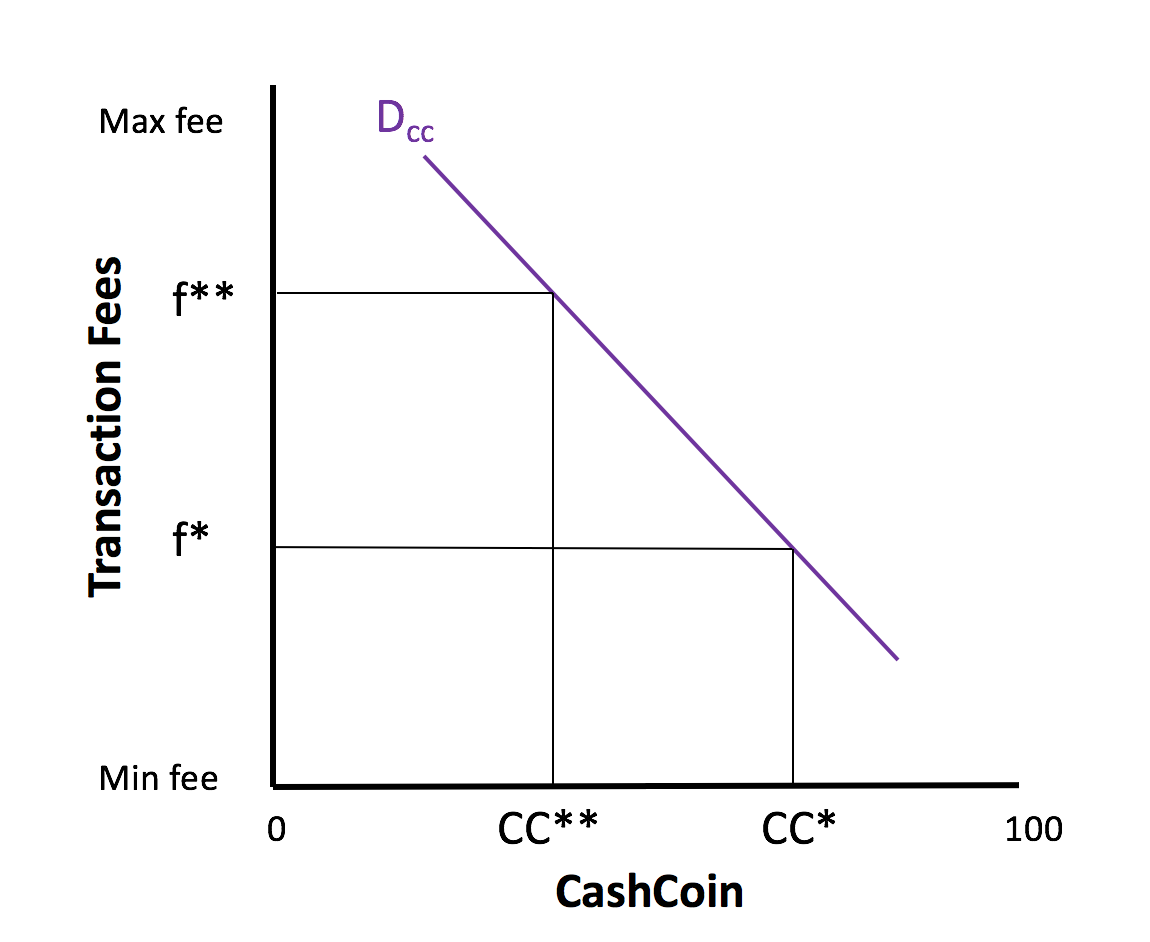
\includegraphics[width=7cm]{dcfc.png}}
\subfigure[Change in demand for CashCoin]{\label{fig32}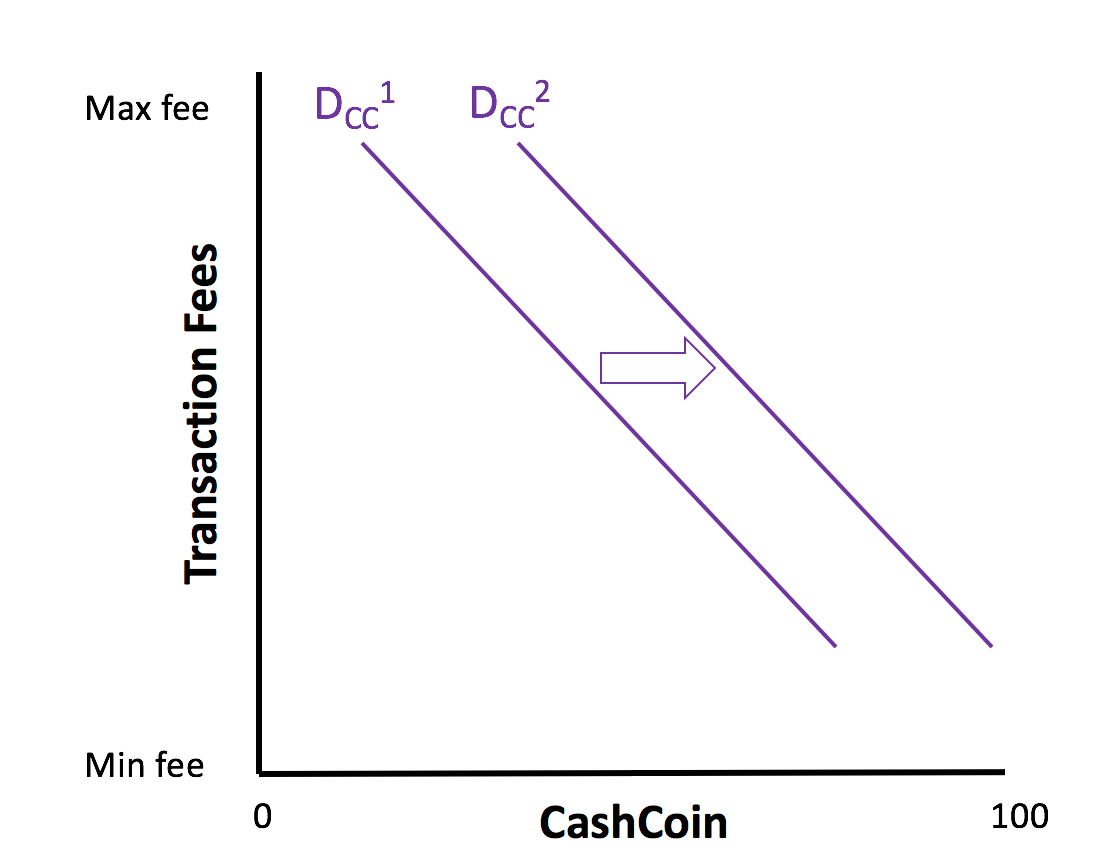
\includegraphics[width=7cm]{cidfc.png}}
\caption{Dynamics of CashCoin}
\end{figure}

The various sources of demand for CashCoins (transactions, precautionary and speculative) will vary negatively with transaction fees. An additional source of demand for CashCoins is from participants wanting lesser decentralization, faster throughputs and lower fees. Let’s label this demand as the higher network performance demand. Lower the fees, higher the demand for CashCoins.

Lets suppose CC** is the total amount of CashCoins at some point in time. I.e., CC** is the supply of CashCoins. Then, the CashCoin market equilibrium will occur at transaction fee f** where the demand meets supply. Now, suppose CashCoin availability increases to CC*, the market equilibrium will occur at transaction fee f* where the demand curve meets the new supply.

\subsection{Change in Demand for CashCoin}

Previously, we have identified 4 sources of demands for CashCoins. i) transactions demand, ii) precautionary demand, iii) speculative demand and iv) higher network performance demand. The various sources of demand for CashCoins can change. For example, during festivals in light of higher retail spending, the transaction demand may rise moving the demand curve as shown in the above figure.

\subsection{Demand Curve for BondCoin}

The various sources of demand for BondCoins (storage, fees and speculative) will vary positively with transaction fees. An additional source of demand for BondCoins is from participants wanting more decentralization and who do not mind paying higher fees. Let’s label this demand as the higher decentralization demand. Higher the fees, higher the demand for BondCoins.

\begin{figure} [!htbp]
\centering    
\subfigure[Demand Curve for BondCoin]{\label{fig33}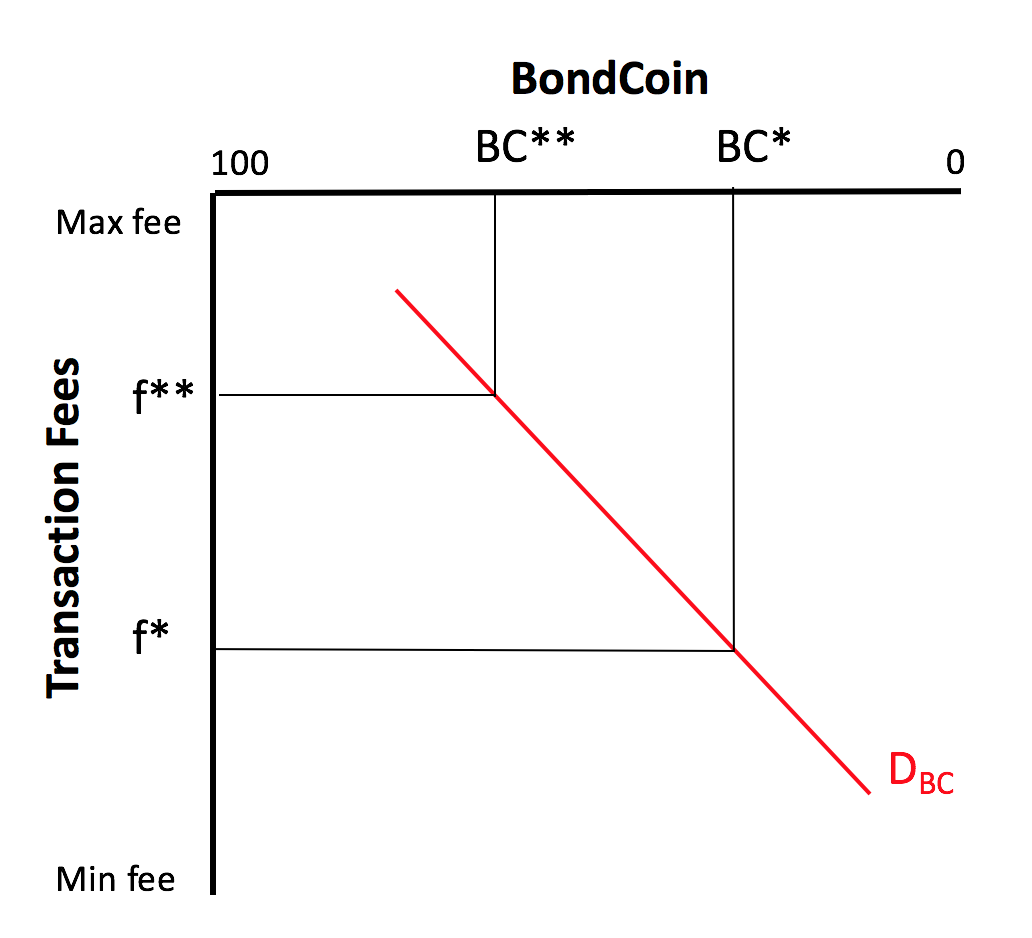
\includegraphics[width=7cm]{dcfb.png}}
\subfigure[Change in demand for BondCoin]{\label{fig34}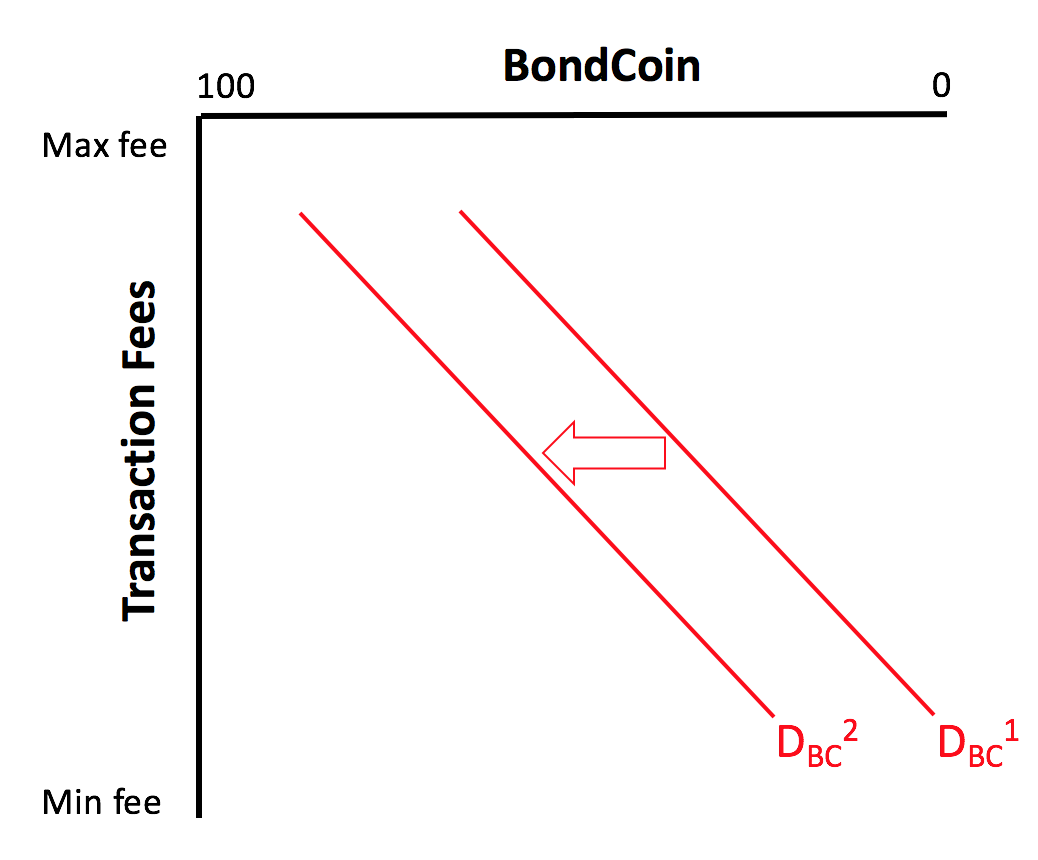
\includegraphics[width=7cm]{cidfb.png}}
\caption{Dynamics of BondCoin}
\end{figure}

Lets suppose BC* is the total number of BondCoins at some point in time. I.e., BC* is the supply of BondCoins. Then, the BondCoin market equilibrium will occur at transaction fee f* where the demand meets supply. Now, suppose BondCoin availability increases to BC**, the market equilibrium will occur at transaction fee f** where the demand curve meets the new supply.

\subsection{Change in Demand for BondCoin}

Previously, we have identified 4 sources of demands for BondCoins. i) storage demand, ii) fees demand, iii) speculative demand and iv) higher decentralization demand. The various sources of demand for BondCoins can change. For example, if the transaction fees increase in anticipation of subdued transaction volumes, the fee demand may rise moving the demand curve as shown in the above figure.

\section{The Common Market Equilibrium}

The supply of BondCoins is simply maxCoins - supply of CashCoins. As shown below, it can be represented by a single line. The supply curve intersects with the demand curves of CashCoin and BondCoin at the same point. This is the common market equilibrium for both CashCoins and BondCoins. There is of course a single fee value f for this common market equilibrium.

\begin{figure}[!htbp]
\centering
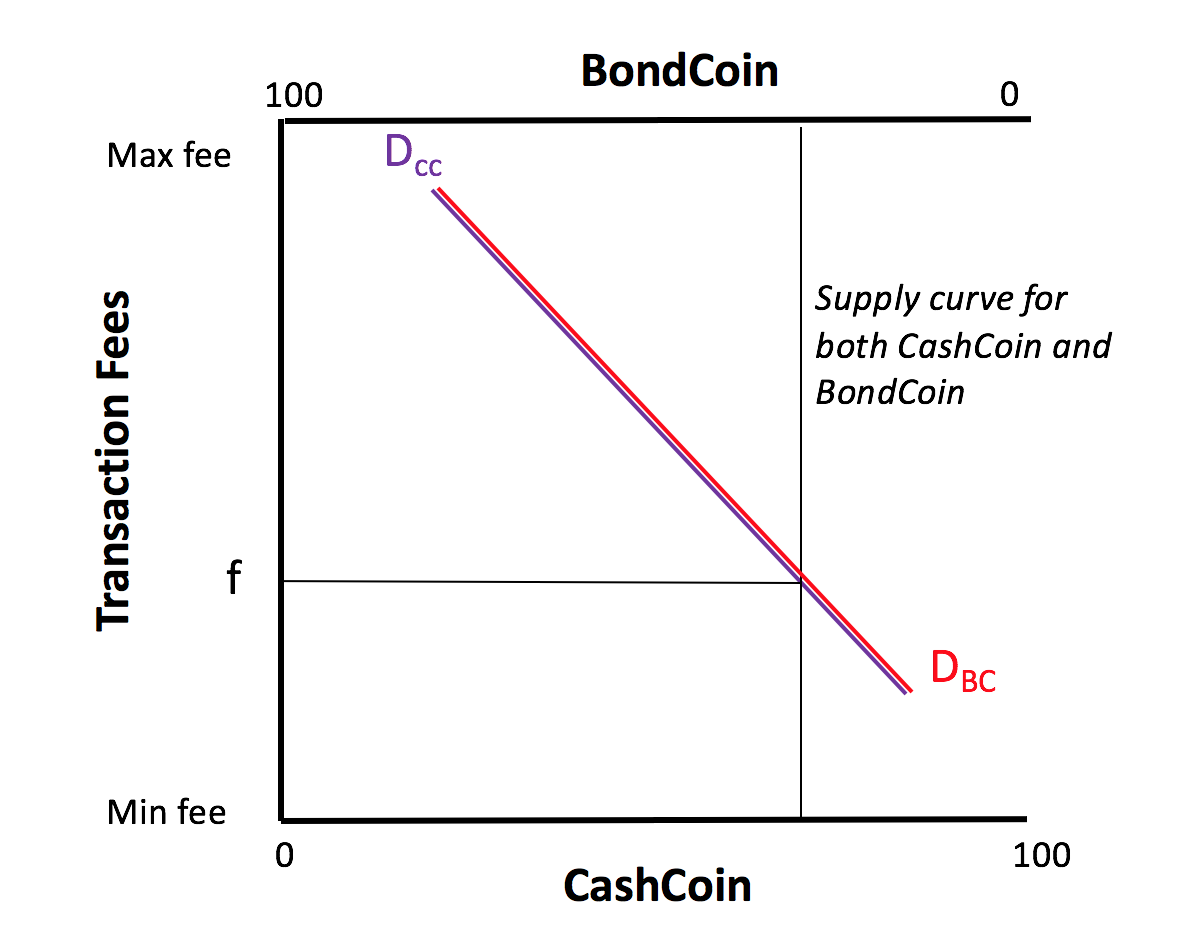
\includegraphics[height=10cm]{tcme.png}
\caption{The Common Market Equilibrium}
\label{fig35}
\end{figure}

This common market equilibrium represents the steady state of the system that respects the aggregate demands and supplies for CashCoin and BondCoin. The number of BondCoins at this equilibrium represent the number of validators in the blockchain.